\subsection{Infrarot Sensor GP2Y0A710K0F}
Diese Messung wird gemeinsam mit Gruppe 39 durchgeführt. \\
Das Modul GP2Y0A710K0F von Sharp ist ein Infrarotsensor, mit welchem Distanzen 
gemessen werden können. Die Messung basiert auf Triangulation. Der Sensor 
beinhaltet eine Infrarot LED (Light emitting diode) mit einer Linse. Das vom 
Objekt reflektierte Licht fällt über eine weitere Linse auf eine Reihe von 
Photoempfängern. Damit wird gemessen, unter welchem Winkel das reflektierte 
Licht auf den Sensor trifft. Die Distanz lässt sich wie folgt berechnen: 
\[ D = d \cdot \arctan(\alpha) \]
\begin{tabular}{@{}ll}
    $D$         & Distanz zum Objekt \\
    $d$         & Abstand der Linsen (38mm) \\
    $\alpha$    & Winkel des zurückreflektierten Lichts gegenüber der Sensorebene \\
\end{tabular} \\
Preislich bewegt sich der Sensor im selben Rahmen wie Ultraschall Module. 

\subsubsection{Eckdaten}
\begin{zebratabular}{ll}
    \rowcolor{gray} Eigenschaft & Wert \\
    Messbereich                 & 1 - 5.5m \\
    Interface                   & Analog \\
    Strombedarf                 & <50mA \\
    Spannung                    & 4.5 - 5.5V \\
\end{zebratabular}

\subsubsection{Testkorb}
Als Testkorb wird der Abfallkorb aus dem Raum C200 verwendet. \\
\begin{zebratabular}{ll}
    \rowcolor{gray} Eigenschaft & Wert \\
    Durchmesser oben    & 38 cm \\
    Durchmesser unten   & 33 cm \\
    Höhe                & 48 cm \\
    Farbe               & schwarz (matt) \\
    Material            & Kunststoff () \\
    Hersteller          & Helit \\
    Typ                 & 61062 \\
\end{zebratabular}

\subsubsection{Messmittel}
\begin{zebratabular}{lll}
    \rowcolor{gray} Gerät &
        Typ &
        Nummer \\
    Speisegerät &
        Hameg ... &
        SN ... \\
    Mainframe &
        Hameg 800? &
        SN ... \\
    Oszilloskop &
        Agilent &
        SN ... \\
    Signalgenerator Servo &
        SM Modellbau Unitest 2 &
        SN: 25494.3 \\
\end{zebratabular} \\
Die Messungen werden im Raum B332c durchgeführt. Die Messstrecke liegt dabei 
auf der ersten Tischreihe. Der Sensor ist am Ende der Wand montiert. 

\subsubsection{Messung Abtastung}
Um die Funktionsweise des Sensors besser zu verstehen, wird zunächst die 
Abtastung des Sensors ermittelt. Dazu wird die ausgesandte Infrarotstrahlung 
mittels einer Photodiode (SFH213) gemessen. Um die Diode zu entladen, wird ein 
Widerstand mit 100 k$\Omega$ parallel an die Diode angeschlossen. 

Die Messung zeigt, dass der Sensor mit Impulspaketen arbeitet. Die Pulse haben 
eine Pulsweite von 155 $\mu$s und eine Periodendauer von 1 ms. Ein Impulspaket 
besteht aus acht Pulsen und wird alle 16 ms wiederholt. Dieser Wert deckt sich 
mit dem vom Hersteller engegebenen Wert von 16.5 ms $\pm$ 3.7 ms. vgl. 
\cite{Datasheet:GP2Y0A710K0F}

\subsubsection{Messung Messgenauigkeit}
Die Messung der Messgenauigkeit wird bei geschlossenen Storen durchgeführt. Zudem 
ist die Beleuchtung bis auf die Tafelbeleuchtung eingeschaltet. Die Werte 
werden aus mindestens 100 Messungen bestimmt. \\
\begin{zebratabular}{lll}
    \rowcolor{gray} Abstand [cm] & Vout (mean) [V] & Std. Dev [mV] \\
    50  & 3.09  & 542 \\
    60  & 3.09  & 1.15 \\
    70  & 2.94  & 6.8 \\
    80  & 2.71  & 10.7 \\
    90  & 2.46  & 19.0 \\
    100 & 2.18  & 27.0 \\
    110 & 2.33  & 11.6 \\
    120 & 1.83  & 26.2 \\
    130 & 1.58  & 23.6 \\
    140 & 1.58  & 29.4 \\
    150 & 1.33  & 30.0 \\
    160 & 1.21  & 33.5 \\
    170 & 0.979 & 44.5 \\
    180 & 0.871 & 32.1 \\
    190 & 0.818 & 24.7 \\
    200 & 0.776 & 26.1 \\
    210 & 0.809 & 24.1 \\
    220 & 0.868 & 29.7 \\
\end{zebratabular} \\
Bei den Messungen zeigt sich, dass das Abtastinterval im Signal sichtbar ist 
und somit nicht gefiltert wird. \\
Ausserdem zeigt sich, dass das Ergebnis stark vom seitlichen 
Versatz des Eimers gegenüber der Sensorachse abhängig ist. 

\subsubsection{Messung Durchfahren eines Objektes}
Der Eimer wird vor dem Sensor durchgefahren. Anschliessend wird der Eimer mit 
weissem Papier beklebt. Der Eimer hat dabei eine Distanz von 2 m zum Sensor. 
Die Wand hinter dem Sensor hat einen Abstand von 2.6 m zum Sensor. 
\begin{figure}[h!]
    \centering
    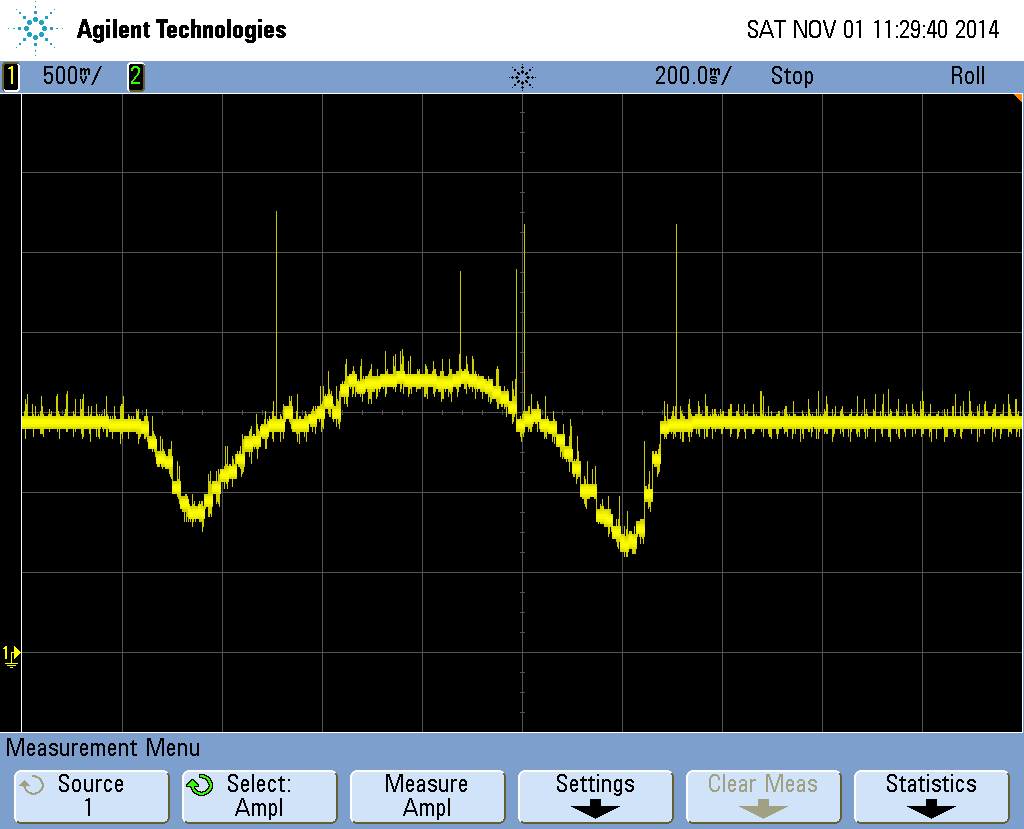
\includegraphics[width=0.4\textwidth]{fig/scope_75.png}
    \caption{Durchfahren mit Schwarzem Korb}
    \label{fig:shift_ir_black}
\end{figure}
\begin{figure}[h!]
    \centering
    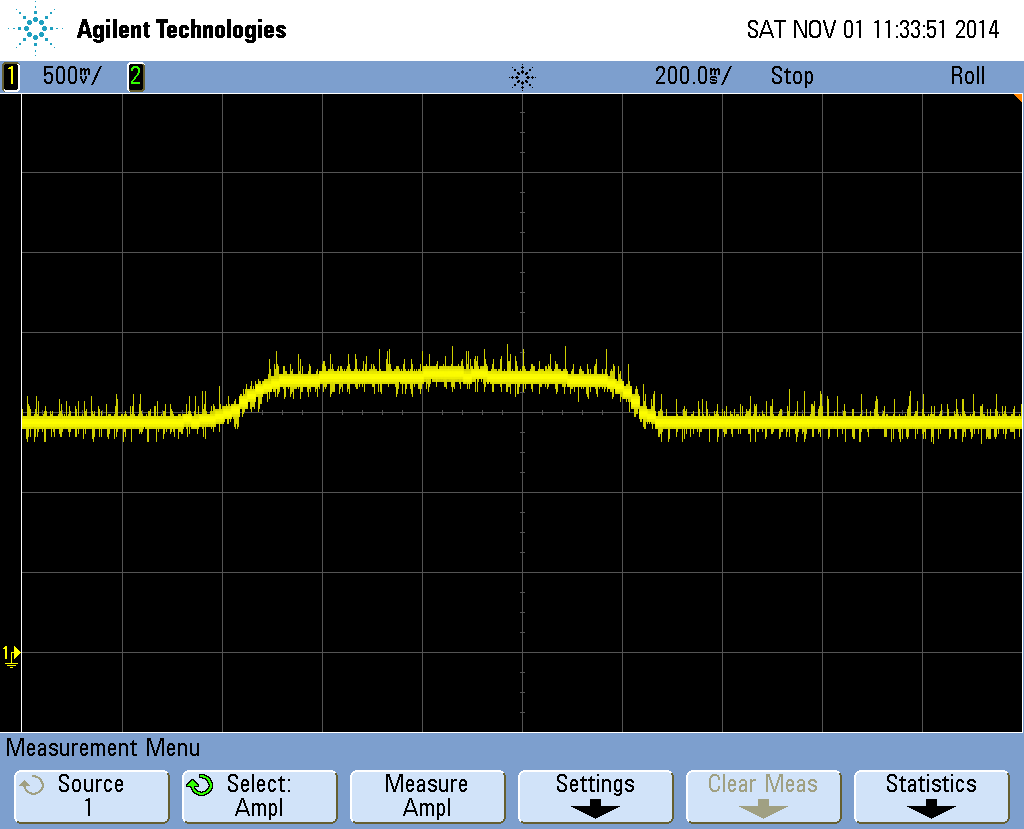
\includegraphics[width=0.4\textwidth]{fig/scope_77.png}
    \caption{Durchfahren mit Weissem Korb}
    \label{fig:shift_ir_white}
\end{figure}

\subsubsection{Messung Scan mit Servomotor}
Als letzter Versuch wird der Sensor auf ein Servo montiert und hin und her 
gedreht. Damit wird ein Scan, wie er in einer Anwendung durchgeführt wird, 
nachgebildet. Die Dauer eines Scans beträgt 0.72 s. Der Abstand zwischen 
Eimer und Sensor beträgt 1.39 m. Die Wand hinter dem Eimer hat eine Distanz 
von 2 m zum Sensor. Auch dieser Versuch wird mit einem schwarzen und mit einem 
weissen Eimer durchgeführt. 
\begin{figure}[h!]
    \centering
    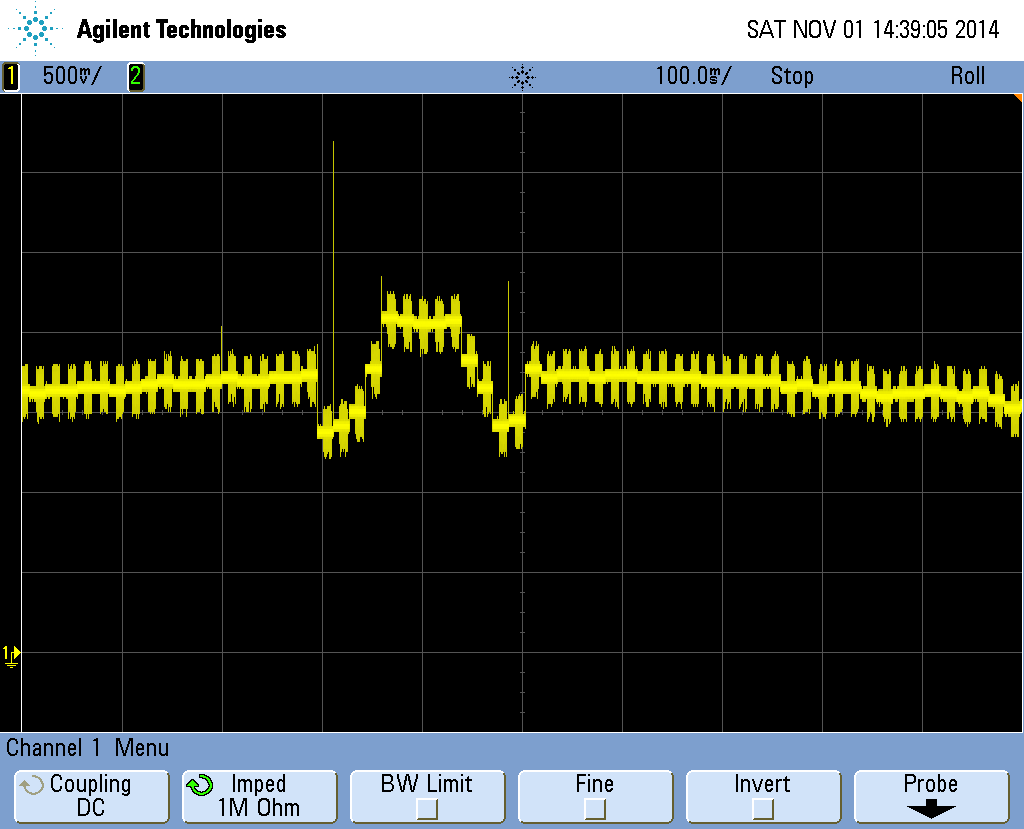
\includegraphics[width=0.4\textwidth]{fig/scope_80.png}
    \caption{Scan mit Schwarzem Korb}
    \label{fig:scan_ir_black}
\end{figure}
\begin{figure}[h!]
    \centering
    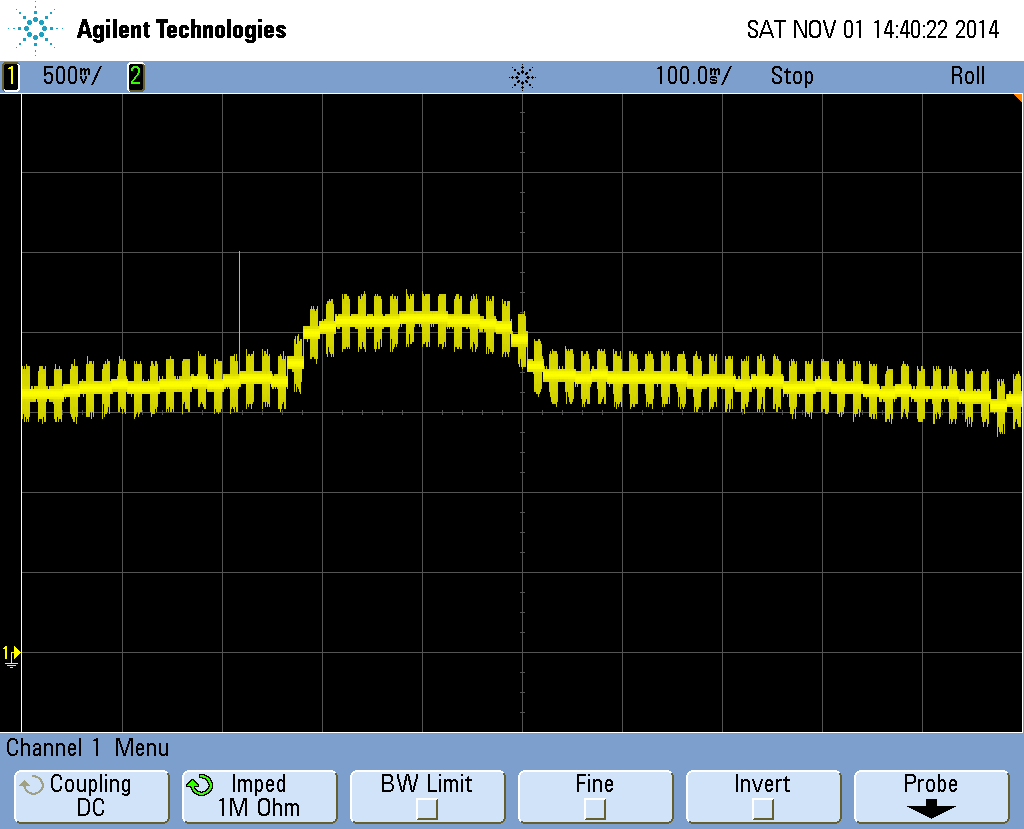
\includegraphics[width=0.4\textwidth]{fig/scope_82.png}
    \caption{Scan mit Weissem Korb}
    \label{fig:scan_ir_white}
\end{figure}
\subsubsection{Fazit der Messungen des Infrarotsensors}
Die ausführlichen Messungen des Infrarotsensors GP2Y0A710K0F führten zum Ergebnis, dass die Korberkennung mittels Infrarot für unser Projekt nicht geeignet ist. Die schwarze Farbe des Korbes bereitet dem Sensor Probleme. Der Korb wird zwar erkannt, doch insbesondere auf den Seiten kann keine genaue Grenze erkannt werden. Die Resultate mit einem weissen Korb waren viel genauer und die Position des Korbes könnte exakter bestimmt werden. Da eine genaue Bestimmung der Position des Korbes für unser Projekt essentiell ist, wird auf die Verwendung eines Infrarotsensors verzichtet.

